\documentclass[a4paper, 12pt]{article}
\usepackage[T1]{fontenc}
\usepackage[utf8]{inputenc}
\usepackage{apacite}
\usepackage{mathptmx}
\usepackage{enumerate}
\usepackage[margin=0.5in]{geometry}
\usepackage{xspace}
\documentclass{article}
\usepackage{tikz} % For flowchart
\usetikzlibrary{shapes.geometric, arrows}
\usepackage{pgfgantt} % For Gantt chart
% Flowchart styles
\tikzstyle{startstop} = [rectangle, rounded corners, minimum width=3cm, minimum height=1cm, text centered, draw=black, fill=red!30]
\tikzstyle{process} = [rectangle, minimum width=3cm, minimum height=1cm, text centered, draw=black, fill=orange!30]
\tikzstyle{arrow} = [thick,->,>=stealth]

\renewcommand{\baselinestretch}{1.0}

\newcommand\nd{\textsuperscript{nd}\xspace}
\newcommand\rd{\textsuperscript{rd}\xspace}
\newcommand\nth{\textsuperscript{th}\xspace} %\th is taken already

\setlength\parindent{0pt} % set paragraph indent to zero

% fill up your name, ID, contribution and paper title here
\author{
Chen Yu Hang (Leader) \quad 1211107973 \quad Problem Statement, Literature Review, References \\
Vishnunanda Surain \quad 241UC241C3 \quad Executive Summary, Research Questions, \\Hypothesis and 
Objectives, and Flowchart of Research Activities\\
Vinnosh Rau A/L Samudram \quad 1211108264 \quad Introduction, 
Expected Results and Impact\\   
Thong Yun Peng \quad 1211107295 \quad Research Methodology, Research Activities and Milestones\\
}
\title{Bias and Fairness in AI}

\begin{document}
\maketitle

\section*{Executive Summary}


As AI becomes increasingly embedded in decision-making across areas like healthcare, lending, and criminal justice, concerns about fairness and bias in these systems have grown. This research focuses on identifying where bias comes from—whether it's in the data, the models, or human involvement—and finding ways to reduce it. We will use tools such as IBM's AI Fairness 360, Google’s What-If Tool, and Microsoft’s Fairlearn to tackle these biases through various techniques that clean up data, adjust models during training, and refine results after training. By combining technical approaches with ethical considerations, we aim to develop AI systems that are not only accurate but also fair and just. The anticipated result is AI models that deliver fairer decisions, helping to reduce the inequalities AI can sometimes reinforce, particularly among marginalized groups.


 
\hfill
\\
\textbf{Keywords:} Bias, Fair AI, Mitigation Strategies, Ethical Technology \\

\section{Introduction}
Artificial Intelligence (AI) has become a critical component in various industries, transforming decision-making processes through automation and machine learning. AI systems are being increasingly used in sectors such as healthcare, finance, hiring, and criminal justice to streamline tasks and make complex decisions efficiently. However, significant concerns have been raised about bias and fairness in these systems. If the data used to train AI models is biased, these systems can unintentionally reinforce societal inequalities. This issue arises because AI models often rely on historical data, which may reflect existing prejudices and systemic biases. According to Kate Crawford, a leading researcher in AI ethics, "data is a reflection of our past, and if that past is discriminatory, then it will have discriminatory outcomes" (Crawford, 2021). The widespread application of AI, coupled with its potential to shape critical decisions, has prompted an increasing focus on understanding and mitigating bias within these systems.

Despite advances in AI research, the issue of bias remains a persistent challenge. Many current studies focus on technical aspects, such as creating fairness-aware algorithms and post-deployment bias detection methods. For instance, Cynthia Dwork, a pioneer in the field of algorithmic fairness, has developed methodologies to create more equitable algorithms, but she also acknowledges that "fairness is a complex and context-dependent issue that cannot be entirely solved by technology alone" (Dwork, 2012). These technical solutions are often insufficient, as they do not fully address the root causes of bias, which may stem from the data collection, preprocessing, or model design phases. Ruha Benjamin, a sociologist and scholar on race and technology, highlights the disconnect between these technical solutions and their real-world impact, particularly on marginalized communities. She argues that "without understanding the societal and structural roots of discrimination, technological fixes will continue to fall short" (Benjamin, 2019).

This research aims to bridge that gap by exploring both the technical and ethical dimensions of AI fairness. By integrating interdisciplinary approaches, it seeks to contribute to the development of AI systems that are not only efficient but also equitable.


\section{Problem Statement}

 Our research focuses primarily on how AI algorithms compile data before making an unbiased and fair decision and ways to improve them. These algorithms, often trained on historical data, can inadvertently reflect and amplify existing societal biases, leading to unfair outcomes in areas such as hiring, lending, and law enforcement. Ensuring fairness in AI systems is imperative to curb discrimination and maintain public trust. However, identifying, mitigating, and preventing bias in AI remains a complex predicament that requires balancing technical solutions with ethical considerations. Developing robust methods to address bias and ensure fairness is essential for creating equitable and trustworthy AI systems.
 
\section{Research Questions, Hypotheses and Objectives}
Minimum of two and maximum of four for each of the research questions, hypotheses, and research objectives. You can use numbering/bullet point to list them out.\\

Research Questions:

1. In what ways do biases in data, algorithms, and human judgment lead to unfair results in AI systems?

2. How do biases in generative AI shape societal perceptions, and what factors contribute to this issue?

3. Are the current methods for reducing bias in AI effective at addressing inequalities?

4. Can tools like AIF360 help promote fairness in AI systems, especially in critical fields like healthcare?\\


Hypotheses:

1. AI models trained on biased data are more likely to perpetuate societal inequalities.

2. Techniques like data preprocessing and post-processing can meaningfully reduce bias in AI.

3. Generative AI is more prone to reinforcing stereotypes because of the biases in its input data.

4. Using fairness-focused tools like AIF360 will lead to more equitable decisions in AI systems.\\

Research Objectives:

1. To uncover the sources of bias in AI systems and understand their effects on decisions.

2. To analyze how well different strategies for reducing bias work in creating fairer outcomes.

3. To examine how biased AI affects society, particularly in areas like healthcare and law enforcement.
 
4. To explore how tools like AIF360 can be applied to reduce bias in AI systems used in real-world scenarios.


\section{Literature Review}
Based on the selected articles, bias and fairness in AI is paramount if humans are to incorporate technology further into daily activities. AI is defined as makers of intellectual machines and programs. The articles focus on the various ways data is compiled and integrated into AI algorithms to aid the decision-making procedure. Machine learning fairness addresses and eliminates algorithmic bias from machine learning models based on sensitive attributes like race, gender, sexual orientation, disability, and socioeconomic class.For instance, a dataset showed females receiving more favorable credit approvals compared to men. Bias in AI can perpetuate and even exacerbate existing inequalities, leading to discrimination against marginalized groups and limiting their access to essential services. In addition, bias in AI can also lead to new forms of discrimination, such as those dependent on skin color, ethnicity, or even physical appearance. The articles disclosed that these data and algorithms can be manipulated, altered and optimised by humans thanks to tools like IBM’s AI Fairness 360, Google’s What-If Tool as well as Microsoft’s Fairlearn, Furthermore, researchers and practitioners have postulated various approaches to alleviate bias in AI. These approaches involve pre-processing data, model selection, and
post-processing decisions. \\ \\

The collective critical analysis of the research papers has their fair share of pros and cons. As a whole, they state the different kinds of biases which plays a pivotal role in the decision-making procedure such as historical bias,
aggregation bias and what not. Besides, they also offer an
accessible explanation of how biases arise in AI algorithms, particularly
through data selection and model training. Furthermore, the paper recommended
a myriad of ways to mitigate AI machine learning which can to be
conducive and pragmatic. However, they lack extensive real-world proof on the effectiveness of the proposed mitigation techniques. Additionally, they don’t
dive into how to apply and assess fairness constraints or use adversarial
debiasing in real-world settings. All in all, further research has to be conducted as well as comprehensive data compilation before concluding. 

\section{Research Methodology}

This section describes the steps involved in the research methodology, including the techniques, models, methods, and algorithms used, along with metrics for evaluation. The methodology integrates technical and ethical perspectives to address the issue of bias in AI systems comprehensively.

\subsection{Overview of Research Methodology}
The research aims to address biases in AI systems by evaluating various mitigation strategies and testing their effectiveness in real-world applications. The approach integrates technical and socio-ethical perspectives to develop a holistic solution for bias and fairness issues in AI. \\

\subsection{Rationale for Method Choices}
The selection of tools like IBM AI Fairness 360, Google What-If Tool, and Microsoft Fairlearn is based on their effectiveness in identifying and mitigating various types of biases in AI systems. These tools provide comprehensive frameworks for detecting bias and implementing fairness constraints. Their real-world applicability and the robust frameworks they offer for bias detection make them ideal for this research.
\\
\subsection{Research Steps}
The methodology follows a series of structured steps aimed at identifying, mitigating, and evaluating bias in AI systems:

\begin{enumerate}
    \item \textbf{Data Collection:} Gather datasets from reliable sources like the UCI Machine Learning Repository, Kaggle, and domain-specific datasets. Ensure data preprocessing by cleaning, normalizing, and handling missing values to maintain dataset quality and reliability. Consider privacy and ethical concerns when collecting sensitive data.

    \item \textbf{Identification of Bias:} Use tools like IBM AI Fairness 360, Google What-If Tool, and Microsoft Fairlearn to detect biases in datasets and AI models, focusing on biases such as historical bias, aggregation bias, and measurement bias.

    \item \textbf{Bias Mitigation Techniques:} The following bias mitigation strategies will be implemented:
    \begin{itemize}
        \item \textit{Pre-processing Methods}: Modify the data before training, such as by reweighting or resampling data to reduce bias.
        \item \textit{In-processing Methods}: Adjust the training algorithms directly, such as using adversarial debiasing to reduce bias during model learning.
        \item \textit{Post-processing Methods}: Modify the model outputs after training, such as recalibrating predictions to ensure fairness.
    \end{itemize}
    
    \item \textbf{Model Training and Evaluation:} Train AI models using both original and mitigated datasets. Models like Logistic Regression, Random Forest, and Neural Networks will be trained. Model performance will be evaluated using metrics like accuracy, Statistical Parity Difference, and Equalized Odds to balance both performance and fairness.

    \item \textbf{Comparative Analysis:} Use statistical methods such as t-tests or ANOVA to compare the performance of the bias-mitigated models against baseline models. This will help quantify the effectiveness of the mitigation techniques.

    \item \textbf{Ethical Evaluation:} Collect feedback from stakeholders, including AI practitioners and affected communities, to assess the ethical implications of each bias mitigation technique. This step ensures that the chosen strategies are socially responsible, beyond just technical effectiveness.
\end{enumerate} 

\subsection{Evaluation Metrics}
The evaluation of bias mitigation techniques will rely on the following metrics:
\begin{itemize}
    \item \textbf{Statistical Parity Difference:} Measures the difference in positive outcome rates between protected and unprotected groups.
    \item \textbf{Equalized Odds:} Assesses whether false positive and false negative rates are equally distributed across different groups.
    \item \textbf{Accuracy:} Measures overall model performance but will be considered alongside fairness metrics to avoid over-optimization at the expense of fairness.
    \item \textbf{False Positive Rate Disparity:} Examines disparities in false positive rates across different demographic groups.
    \item \textbf{Equal Opportunity Difference:} Evaluates whether the true positive rate is equal across different groups.
\end{itemize}

\subsection{Potential Limitations and Mitigation}
While bias mitigation techniques are promising, they come with limitations:
\begin{itemize}
    \item \textbf{Computational Costs:} Some methods, particularly in-processing techniques like adversarial debiasing, are computationally expensive. This will be mitigated by selecting models and algorithms optimized for efficiency.
    \item \textbf{Data Distortion:} Pre-processing techniques such as reweighting may distort the original dataset. Care will be taken to ensure minimal alteration while maximizing fairness.
    \item \textbf{Real-world Applicability:} Some techniques may work well in controlled environments but may face challenges in real-world deployment. To address this, real-world testing and stakeholder feedback will be integrated into the methodology.
\end{itemize}

\subsection{Visual Representation of Methodology}
The research methodology will be summarized in a flowchart, detailing the sequence from data collection to ethical evaluation. This visual representation will clarify the workflow and inter-dependencies between steps.

\subsection{Ethical Considerations}
An essential aspect of this research is the ethical evaluation of bias mitigation strategies. Stakeholder feedback, including input from marginalized communities, will be collected through surveys or interviews. This ensures that the AI systems are not only technically sound but also align with ethical standards such as fairness, transparency, and accountability.

\begin{table}[h]
    \centering
    \caption{Comparison of Bias Mitigation Techniques}
    \begin{tabular}{|l|p{4cm}|p{3cm}|p{3cm}|p{3cm}|}
        \hline
        \textbf{Technique} & \textbf{Description} & \textbf{Advantages} & \textbf{Disadvantages} & \textbf{Example Application} \\
        \hline
        Pre-processing & Modifies data before training, e.g., reweighting samples & Easy to implement & Can distort original data & Healthcare data rebalancing \\
        \hline
        In-processing & Changes the algorithm during training, e.g., adversarial debiasing & Directly addresses bias during learning & Computationally intensive & Fair neural network training \\
        \hline
        Post-processing & Adjusts predictions after training & Doesn’t alter the model & Less control over decision-making & Credit approval recalibration \\
        \hline
    \end{tabular}
    \label{table:mitigation_techniques}
\end{table}

\section{Research Activities and Milestones}

This section describes the research activities and their timeline. The flowchart illustrates the sequence of activities, while the Gantt chart provides a clear timeline for completing each task within 7 weeks.

\subsection*{Flowchart of Research Activities}

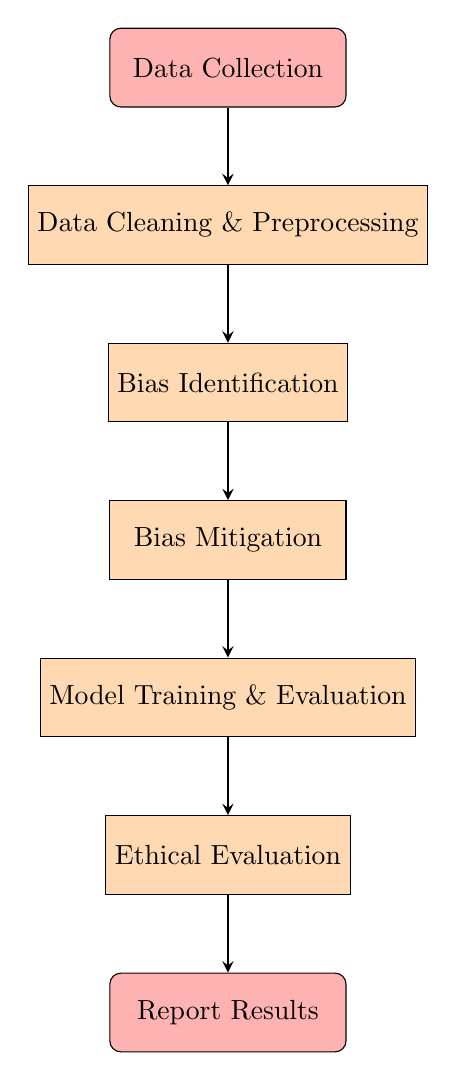
\begin{tikzpicture}[node distance=2cm]

% Nodes for Flowchart
\node (start) [startstop] {Data Collection};
\node (cleaning) [process, below of=start] {Data Cleaning \& Preprocessing};
\node (biasid) [process, below of=cleaning] {Bias Identification};
\node (mitigation) [process, below of=biasid] {Bias Mitigation};
\node (modeltrain) [process, below of=mitigation] {Model Training \& Evaluation};
\node (ethicseval) [process, below of=modeltrain] {Ethical Evaluation};
\node (end) [startstop, below of=ethicseval] {Report Results};

% Arrows for Flowchart
\draw [arrow] (start) -- (cleaning);
\draw [arrow] (cleaning) -- (biasid);
\draw [arrow] (biasid) -- (mitigation);
\draw [arrow] (mitigation) -- (modeltrain);
\draw [arrow] (modeltrain) -- (ethicseval);
\draw [arrow] (ethicseval) -- (end);

\end{tikzpicture}

% Explanations for Flowchart
\subsection*{Explanations of the Research Activities}
1. \textbf{Data Collection:} Gather data from reliable sources to ensure it is diverse and representative. \\
2. \textbf{Data Cleaning \& Preprocessing:} Remove errors and inconsistencies to prepare the data for model training. \\
3. \textbf{Bias Identification:} Use tools like IBM AI Fairness 360 to detect biases in data and models. \\
4. \textbf{Bias Mitigation:} Reduce bias by adjusting data, algorithms, or model outputs. \\
5. \textbf{Model Training \& Evaluation:} Train the AI model using refined data and evaluate it for performance and fairness. \\
6. \textbf{Ethical Evaluation:} Gather feedback from stakeholders to ensure the model is fair and ethically sound. \\
7. \textbf{Reporting Results:} Share findings on bias mitigation, model performance, and ethical considerations.

\subsection*{Gantt Chart for Research Timeline}
The Gantt chart below outlines the timeline for the project, spanning 7 weeks. Each task is mapped to a specific week, and milestones indicate key achievements.

\begin{ganttchart}[
    y unit chart=1cm, % Increase row height (default is 0.8cm)
    x unit=1.2cm,     % Increase column width (default is 0.5cm)
    vgrid, hgrid,     % Adds vertical and horizontal grid lines
    title label font=\bfseries\footnotesize, % Title font settings
    title label anchor/.append style={below=-1.6ex}, % Title position
    title left shift=.05, title right shift=-.05,
    bar/.append style={fill=cyan!80}, % Bar color (adjust as needed)
    bar height=0.8      % Increase bar height (default is 0.6)
]{1}{7}  % Defines the Gantt chart to span 7 weeks
  % Title of the chart (spanning 7 weeks)
  \gantttitle{Research Schedule (Weeks)}{7} \\
  % Labels the weeks
  \gantttitlelist{1,...,7}{1} \\

  % Tasks (Task name) [Start week]{Duration in weeks}
  \ganttbar{Data Collection}{1}{1} \\      % Task lasting 1 week
  \ganttbar{Preprocessing}{2}{2} \\        % Task lasting 1 week
  \ganttbar{Bias Identification}{3}{3} \\  % Task lasting 1 week
  \ganttbar{Bias Mitigation}{4}{5} \\      % Task lasting 2 weeks
  \ganttbar{Model Training}{6}{6} \\       % Task lasting 1 week
  \ganttbar{Ethical Evaluation}{7}{7} \\   % Task lasting 1 week

  % Milestones (add after key tasks)
  \ganttmilestone{Data Collection Complete}{1} \\  % Milestone after week 1
  \ganttmilestone{Bias Mitigation Complete}{5} \\  % Milestone after week 5
  
  % Dependencies (arrows between tasks)
  \ganttlink{elem0}{elem1} % Data Collection -> Preprocessing
  \ganttlink{elem1}{elem2} % Preprocessing -> Bias Identification
  \ganttlink{elem2}{elem3} % Bias Identification -> Bias Mitigation
  \ganttlink{elem3}{elem4} % Bias Mitigation -> Model Training
  \ganttlink{elem4}{elem5} % Model Training -> Ethical Evaluation

\end{ganttchart}
\section{Expected Results and Impact}

 \textbf{Improved Understanding of Bias Origins:} The analysis will uncover the various sources of bias in AI systems, including those embedded in the data, algorithms, and human decision-making processes. This will lead to a deeper comprehension of how biases manifest in real-world AI applications.

 \textbf{Effectiveness of Mitigation Strategies:} The study will provide a comparative analysis of different bias mitigation techniques (pre-processing, in-processing, and post-processing), evaluating their effectiveness in enhancing fairness across AI models in critical areas such as healthcare and criminal justice.
 
\textbf{Role of Fairness Tools:} By applying tools like IBM AI Fairness 360 and Microsoft Fairlearn, the research will demonstrate the practicality and limitations of these tools in addressing bias in real-world scenarios. This will offer actionable insights into how these tools can be integrated into AI development workflows to ensure fairness. 

%References
\bibliographystyle{apacite}
\bibliography{MyBib}
\begin{itemize}
    \item Lory Seraydarian (2023), Bias and Fairness in AI Algorithms, plat.ai/blog/bias-and-fairness-in-ai-algorithms/ 
    \item Luca CM Melchionna (2023), Bias and Fairness in Artificial Intelligence, nysba.org/bias-and-fairness-in-artificial-intelligence/ 
    \item Emilio Ferrara (2023), Fairness And Bias in Artificial Intelligence: A Brief Survey of Sources, Impacts, And Mitigation Strategies, arxiv.org/pdf/2304.07683
    \item Jpn J Radiol (2024), Fairness of artificial intelligence in healthcare: review and recommendations, www.ncbi.nlm.nih.gov/pmc/articles/PMC10764412/
    \item Crawford, K. (2021). \textit{Atlas of AI: Power, Politics, and the Planetary Costs of Artificial Intelligence}. Yale University Press. 
    \item Dwork, C. (2012). \textit{Fairness Through Awareness}. Proceedings of the 3rd Innovations in Theoretical Computer Science Conference (ITCS '12). 
    \item Benjamin, R. (2019). \textit{Race After Technology: Abolitionist Tools for the New Jim Code}. Polity Press. 
\end{itemize}

\end{document}


